%
% Complete documentation on the extended LaTeX markup used for Insight
% documentation is available in ``Documenting Insight'', which is part
% of the standard documentation for Insight.  It may be found online
% at:
%
%     http://www.itk.org/

\documentclass{InsightArticle}

\usepackage[dvips]{graphicx}
\usepackage{multirow}

%%%%%%%%%%%%%%%%%%%%%%%%%%%%%%%%%%%%%%%%%%%%%%%%%%%%%%%%%%%%%%%%%%
%
%  hyperref should be the last package to be loaded.
%
%%%%%%%%%%%%%%%%%%%%%%%%%%%%%%%%%%%%%%%%%%%%%%%%%%%%%%%%%%%%%%%%%%
\usepackage[dvips,
bookmarks,
bookmarksopen,
backref,
colorlinks,linkcolor={blue},citecolor={blue},urlcolor={blue},
]{hyperref}


%  This is a template for Papers to the Insight Journal.
%  It is comparable to a technical report format.

% The title should be descriptive enough for people to be able to find
% the relevant document.
\title{Anomalous Diffusion Paradigm for Image Denoising Process}

%
% NOTE: This is the last number of the "handle" URL that
% The Insight Journal assigns to your paper as part of the
% submission process. Please replace the number "1338" with
% the actual handle number that you get assigned.
%
\newcommand{\IJhandlerIDnumber}{3565}

% Increment the release number whenever significant changes are made.
% The author and/or editor can define 'significant' however they like.
\release{0.1}

% At minimum, give your name and an email address.  You can include a
% snail-mail address if you like.
\author{Antonio Carlos da S. Senra Filho$^{1,2}$ and Luiz Ot\'{a}vio Murta Junior$^{1}$}
\authoraddress{$^{1}$University of Sao Paulo, Brazil\\
               $^{2}$King's College London, United Kingdom}

\begin{document}

%
% Add hyperlink to the web location and license of the paper.
% The argument of this command is the handler identifier given
% by the Insight Journal to this paper.
%
\IJhandlefooter{\IJhandlerIDnumber}


\ifpdf
\else
   %
   % Commands for including Graphics when using latex
   %
   \DeclareGraphicsExtensions{.eps,.jpg,.gif,.tiff,.bmp,.png}
   \DeclareGraphicsRule{.jpg}{eps}{.jpg.bb}{`convert #1 eps:-}
   \DeclareGraphicsRule{.gif}{eps}{.gif.bb}{`convert #1 eps:-}
   \DeclareGraphicsRule{.tiff}{eps}{.tiff.bb}{`convert #1 eps:-}
   \DeclareGraphicsRule{.bmp}{eps}{.bmp.bb}{`convert #1 eps:-}
   \DeclareGraphicsRule{.png}{eps}{.png.bb}{`convert #1 eps:-}
\fi


\maketitle


\ifhtml
\chapter*{Front Matter\label{front}}
\fi


% The abstract should be a paragraph or two long, and describe the
% scope of the document.
\begin{abstract}
\noindent
Anisotropic and isotropic diffusion equations have been extensively applied on biomedical image processing for many years and a great diversity of algorithm have been proposed by the scientific community. Here, it is available a recent new implementation of the anomalous diffusion equation, based on the Fokker-Planck PDE diffusion equation (also known as the Porous Media equation). The major contribution of the anomalous process in the image processing area is the possibility to regulates a sub or super-diffusion characteristic in the noise attenuation problem, which have been showed as a suitable solution for the preservation of fine details in complex objects such as the human brain. An ITK Module is offered here in order to easily add the Anisotropic Anomalous Diffusion (AAD) and Isotropic Anomalous Diffusion (IAD) filters in the ITK hierarchy.

% implemented using the Insight Toolkit
% ITK \url{www.itk.org}. The code of the algorithm is written following the
% ITK CodingStyle as described in the directory
% 
% \code{ITK/Documentation/Style.pdf}
% 
% This paper is accompanied with the source code, input data, parameters and
% output data that the authors used for validating the algorithm described in
% this paper. This adheres to the fundamental principle that scientific
% publications must facilitate reproducibility of the reported results.

\end{abstract}

\IJhandlenote{\IJhandlerIDnumber}

\tableofcontents

\section{Brief Introduction About Anomalous Diffusion Process}

Diffusion process is widely applied to digital image enhancement both directly introducing diffusion equation as in anisotropic diffusion (AD) filter, and indirectly by convolution as in Gaussian filter. Anomalous diffusion process (ADP), given by a nonlinear relationship in diffusion equation and characterized by an anomalous parameters $q$, is supposed to be consistent with inhomogeneous media. 

The anomalous diffusion process (ADP) is a natural transport approach that occurs in complex media, leading to exponential variance evolution in time \cite{Tsallis2009Livro}. ADP generalizes classical diffusion by introducing a power law in the heat flow equation, and is reasonably more adequate for complex media, e.g. biological media \cite{Hagmann2006} and theoretical physics \cite{Lenzi2003}. ADP could be mathematically denoted by a power law in the Fokker-Planck equation, leading to the generalized form presented in Equation (\ref{Eq:PorousMedia}). There are several generalizations of the Fokker-Plank equation, which should give many different PDEs. Here we adopt only the so called porous media form, allowing the super-diffusive and the sub-diffusive processes. Equation (\ref{Eq:PorousMedia}) shows the generalized heat flow equation that is the main PDE equation for the anomalous diffusion paradigm. This equation is the basis for the Anisotropic Anomalous Diffusion (AAD) and Isotropic Anomalous Diffusion filters (IAD).

\begin{equation}\label{Eq:PorousMedia}
 \frac{\partial \rho}{\partial t} = \nabla.[D_{q}.\nabla \rho]^{2-q}
\end{equation}

Where $\rho$ represents diffusing element concentration, $D_{q}$ denotes the generalized diffusion coefficient and $q$ is the power law parameter conveniently written. When $q = 1$, the Equation (\ref{Eq:PorousMedia}) recovers classical diffusion, for $q < 1$ it represents sub-diffusive process, and when $q > 1$ it means super-diffusive phenomena are present \cite{Tsallis2009Livro,Schwammle2008}. $D_{q}$ is the diffusion coefficient function that regulates diffusibility. We can distinguish $D_{q}$ function in isotropic: when the diffusion coefficient is the same for all direction, i.e. $D_{q}$ is direction invariant; and anisotropic behavior: when $D_{q}$ is driven to specific directions, similar to Perona and Malik approach.

In fact, the AAD and IAD filter share a comparable behavior with the Perona and Malik anisotropic filtering method and Gaussian smoothing, respectively. However, the major difference between the anomalous and classical approach is the $q$ value, which allow us to define super and sub diffusion process into the local voxel weghting. Figure \ref{Fig:ExamplesImages} illustrates a simple example of MRI brain images filtered from each method for $q<1$ (sub-diffusive process), $q=1$ (classical process) and $q>1$ (super-diffusive process).

\begin{figure*}[ht]
\centering
%\textbf{a)}
 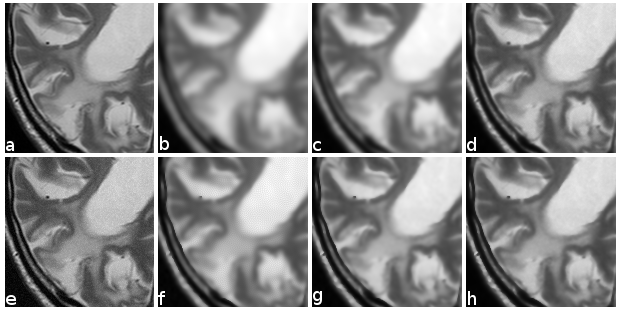
\includegraphics[width=16cm]{Img/figure5.png}
\caption{Examples of the obtained visual qualities with different q values and filtering approaches. \textbf{a} is the original image without additive noise and \textbf{e} is the image with non central $\chi$ noise of 15\% intensity added. \textbf{b}, \textbf{c} and \textbf{d} show the effect of IAD filtering for $q = 0.7$, $q = 1.0$ and $q = 1.5$, respectively. \textbf{f}, \textbf{g} and \textbf{h} show the effect of AAD filtering for $q = 0.7$, $q = 1.0$ and $q = 1.5$, respectively. Notice that the anomalous filters with $q = 1.5$ are more effective in preserving the structure edges and maintaining an effective noise filtering for the observed images regions than the classical AD filter ($q = 1.0$). The $q$ value with a non optimum filtering behavior ($q = 0.7$), intentionally used to illustrate the importance of the q parameter.}
\label{Fig:ExamplesImages}
\end{figure*}

More details about the theory of anomalous diffusion and the image filter implementation could be found in \cite{SenraFilho2015} and some recent publications made with both image filtering methods could be seen in \cite{Filho2014b,Filho2014,Filho2014a,SenraFilhoCBEB2014,SenraFilho_EMBC2013,Filho2014c}.

\section{Module Description}

\subsection{Filters Implementation}

Proposed IAD and AAD filters are based on iterative numerical algorithms for ADP. The method used to solve partial differential anomalous equations uses finite differences, of first and second order, when time and space becomes discrete, i.e. digital images. Both isotropic and anisotropic approaches were implemented through numerical differential operators using explicit numeric formulation, similar to AD filter \cite{PERONA1990}. 

Numerical approaches were implemented using differential operators in one dimension, and then rotated in eight angle directions with respect to the central reference pixel. We can express this rotation in Equation (\ref{Eq:NumericDiff}).

\begin{equation}\label{Eq:NumericDiff}
I_{\phi,t+1}=I_{\phi,t}+\lambda . \nabla [D_{q}.\nabla I_{\phi,t}^{2-q}]
\end{equation}

Where $I_{\phi,t}$ and $I_{\phi,t+1}$ are the evaluated images in $t_i$ iterations, and $I_{\phi,0}$ is the original image. $D_q$ is the diffusion coefficient regulated by a power law with $q$ \cite{Schwammle2008}, and $\phi$ are the possible orientations with respect to the central pixel. Equation (\ref{Eq:NumericDiff}) assumes the time step constant \cite{PERONA1990} ($\lambda \propto \Delta t/\Delta x^{2}$) and it depends on the numerical discretization. A careful time step determination plays an important role for numerical stability \cite{PERONA1990}. The time step determination have a direct influence on the numeric discretization of the diffusion equation and here it follows the same assumptions made for the classical anisotropic diffusion algorithm \cite{PERONA1990}. More details about the time step parameters and numerical stability can be found in \cite{SenraFilho2015,PERONA1990}.

The AAD filtering approach was proposed to regulate the diffusion intensity at the edge neighborhoods by an edge stop function, i.e. the diffusion coefficient is attenuated at image gradients $g(∣\nabla I∣)$. For AAD filters, i.e. parametric values $q \neq 1$, the maximum values considered for $D_q$ are the same found for the IAD filter due to the diffusion intensity stability. The diffusion coefficient for each pixel in the images follows the edge preserving function $g(∣\nabla I∣)$ considering limits estimated by the function described in Equation (\ref{Eq:CoeffDGeneralized}). The edge preserving stop function has the form given by Equation (\ref{Eq:gFunction}).

The generalized diffusion coefficient value, $D_q$, must be consistent with ADP so that it can be used in IAD and AAD filters \cite{Schwammle2008}. The analytical form for $D_q$ must be consistent with the ADP time evolution of variance, which follows $\sigma^{2} = 2.D_q.t$, i.e. linear relationship for classical diffusion, and $\sigma^2 \propto t^{2/(3 - q)}$, i.e nonlinear relationship for ADP \cite{Tsallis2009Livro}. One can deduce a generalized $D_q$ given by Equation (\ref{Eq:CoeffDGeneralized}):

\begin{equation}\label{Eq:CoeffDGeneralized}
D_q = 
\begin{cases}
  \frac{1}{2}.\alpha^{\frac{2}{3-q}}.\Big(\sqrt{\frac{(1-q)}{\pi}}.\frac{\Gamma (1 + \frac{1}{1 - q})}{\Gamma (\frac{3}{2} + \frac{1}{1-q})}\Big)^{\frac{2-2q}{3-q}}  & q < 1 \\
	  \frac{1}{2}.\alpha & q = 1 \\
	  \frac{1}{2}.\alpha^{\frac{2}{3-q}}.\Big(\sqrt{\frac{(q-1)}{\pi}}.\frac{\Gamma (\frac{1}{q-1})}{\Gamma (\frac{1}{q-1} - \frac{1}{2})}\Big)^{\frac{2-2q}{3-q}}  & 1 < q < 2
	  
\end{cases}
\end{equation}

\begin{equation}\label{Eq:gFunction}
  D_q(\overrightarrow{x},t)=D_q.g(|\nabla I_{x}|)=D_q. exp\Big[ -\Big( \frac{\nabla I_{x}}{\kappa}\Big)^{2} \Big]
\end{equation}

Where $\alpha = (2 - q)(3 - q)$. When $q \neq 1$ Equation (\ref{Eq:CoeffDGeneralized}) denotes the diffusion coefficient ($D_q$) that is consistent with \textit{q-Gaussian} probability distributions \cite{Tsallis2009Livro}. Since we can have lower diffusion coefficients, the function in Equation (\ref{Eq:CoeffDGeneralized}) represents the upper limit for $D_q$, i.e. maximum coefficient applicable for image spaces. Note that for classic diffusion equation, i.e. $q = 1$, the diffusion coefficient $D_1$ applied to images lies in the range $0 \leq D_1 \leq 1$. Equation (\ref{Eq:CoeffDGeneralized}) was rewritten from \cite{Schwammle2008} and adapted for numeric form.

We present the numerical algorithm for one dimension showing only x-axis for a better visualization. The method can be generalized to higher dimensions with the appropriate considerations for the filter parameters definition due to possible numeric instability. The convergence, stability and consistence are issues that must be carefully studied for different numerical discretization. The numeric algorithm for the IAD filter is summarized in Equation (\ref{Eq:IsoAnomNumericFormAnomalous}) and for the AAD filter in Equation (\ref{Eq:AnisoAnomNumericFormAnomalous}).

\begin{eqnarray}\label{Eq:IsoAnomNumericFormAnomalous}
 I_{x,t+1} &=& I_{x,t} + \lambda.\Big[ D_q. \nabla^2 I_{x,t}^{2 - q} )\Big] \nonumber \\
  &=& I_{x,t} + \lambda.\Big[ D_q. ( I_{x - 1,t}^{2 - q} - 2.I_{x,t}^{2 - q} + I_{x + 1,t}^{2 - q} )\Big]
\end{eqnarray}

\begin{equation}\label{Eq:AnisoAnomNumericFormAnomalous}
 I_{x,t+1} = I_{x,t} + \lambda.\Big[ D_q(x+\frac{\Delta x}{2},t) . \nabla_{E} I_{x,t} + D_q(x-\frac{\Delta x}{2},t). \nabla_{W} I_{x,t}) \Big]
\end{equation}

The sub-scripts \textit{N, S, E, W} denote cardinal directions and this approach are similar to the classical anisotropic filter method as described by the classical anisotropic filtering

\begin{eqnarray}\label{Eq:FiniteDiffGrad}
 \nabla_{N} I_{x,y} &=& I_{x,y - 1} - I_{x,y} \nonumber \\
 \nabla_{S} I_{x,y} &=& I_{x,y + 1} - I_{x,y} \nonumber \\
 \nabla_{E} I_{x,y} &=& I_{x + 1,y} - I_{x,y} \nonumber \\
 \nabla_{W} I_{x,y} &=& I_{x - 1,y} - I_{x,y}  
\end{eqnarray}

\subsection{Module Classes}

The \code{ITKAnomalousDiffusionFilters} module provides two implementations of anomalous diffusion process, which are denoted as the \code{itkAnisotropicAnomalousDiffusionImageFilter} and \code{itkIsotropicAnomalousDiffusionImageFilter}. Each filter has its own characteristics over the output results obtained in a multidimensional data, which the parameters set needed for each algorithm is explained below.

\subsubsection{Parameters}\label{Sec:Parameters}

In general, there are a common set of parameters which can be used for both anisotropic and isotropic filters. In this case, the \code{SetIterations()}, \code{SetQ()} and \code{SetTimeStep()} are shared in both methods. The \code{SetCondutance()} parameter should be adjusted in the AAD filter case and the \code{SetGeneralizedDiffusion()} parameter should be adjusted in the IAD filter case. 

% \begin{itemize}
\paragraph{Condutance}
 This parameter takes the control of Equation (\ref{Eq:gFunction}), which directly sets the $\kappa$ variable. This edge function is responsible to define what would be the filter criteria to preserve the image object’s frontiers. A higher value of \code{Condutance} will result in a strong smoothness around the background/foreground areas, revealing a strong edge delimitation between structures. On the contrary, a lower value of \code{Condutance} will result in a less disturbance in the general structure shapes, but with lower noise attenuation too. This parameter is only used in \code{itkAnisotropicAnomalousDiffusionImageFilter} method. Values around $5.0\sim20.0$ should be fine for the majority of applications.

 \paragraph{GeneralizedDiffusion}
 This parameter has a correspondence behavior with the \code{Condutance} parameter, but in relation to the \code{itkIsotropicAnomalousDiffusionImageFilter} method. This parameter regulates the $D_q$ variable as seen in Equation (\ref{Eq:IsoAnomNumericFormAnomalous}) which in a practical way defines how large is the \textit{q-Gaussian} variability ($\sigma^{2}$). One may note that the $D_q$ is also presented in Equation (\ref{Eq:AnisoAnomNumericFormAnomalous}), but our implementation maintains it fixed at the $max[D_q(r,t)]$ for the \code{itkAnisotropicAnomalousDiffusionImageFilter} method.
 
 \paragraph{TimeStep}
 The time step variable is only a numerical constant that imposes a numerical stability to both diffusion equations. Its constraints are defined in \cite{SenraFilho2015, PERONA1990} and is closely related to the image dimension used. Both methods in \code{ITKAnomalousDiffusionFilters} module checks at the execution time if the \code{TimeStep} value where set properly.
 
 \paragraph{Iterations}
 The number of iterations is responsible to set the time evolution in the numerical PDE, in both diffusion paradigms. In other words, this parameter is responsible to define how strong will be the smoothness of the whole image due to iterative update. Usually, an \code{Iterations} value around $5\sim10$ could fit properly for the majority of MRI structural images.
 
 \paragraph{Q}
 The anomalous parameter, or $Q$, is the major parameter to set the type of probability distribution that should be applied in the filtering procedure. In summary, this parameter regulates the sub and super diffusion process in the whole image and should be well adjusted depending on the type of noise and image quality used. More details about the \textit{q-Gaussian} probability distribution family could be found in \cite{Tsallis2009Livro,Schwammle2008}. In \cite{SenraFilho2015} it was found a value of $Q\sim1.5$ as the optimum case for MRI structural brain images. However, it is important to apply a previous parameters evaluation beforehand the final application in your image dataset.
 

\section{Practical Example}

The following example illlustrates a simple usage of the \code{itkAnisotropicAnomalousDiffusionImageFilter} class. The same implementation could be replicated with the \code{itkIsotropicAnomalousDiffusionImageFilter} approach.

Initally, for this example, we start declaring the basic classes that will be used for data reading, writing and processing

\small
\begin{verbatim}
#include "itkImage.h"
#include "itkImageFileReader.h"
#include "itkImageFileWriter.h"
#include "itkAnisotropicAnomalousDiffusionImageFilter.h"
\end{verbatim}
\normalsize

After that, the \code{main()} function could be initiated

\small
\begin{verbatim}
int main(int argc, char* argv[])
{
    const unsigned int Dimension = 3;

    typedef float                       PixelType;
    typedef float                       PixelOutType;
    typedef itk::Image<PixelType, Dimension>    ImageType;

    typedef itk::ImageFileReader<ImageType> ReaderType;
    typedef itk::ImageFileWriter<ImageType> WriterType;
\end{verbatim}
\normalsize

It is important to say that both image filters are capable to process multidimensional data, which in this example it was set to \code{Dimension = 3}. Furthermore, it is important to highlight the \code{PixelType} and \code{PixelOutType}, that defines the type of data expected as input and output, where it should be set to \code{float} type in order to not restrict the local weighting estimative due to data precision. Since the majority of biomedical data are encoded using double precision data types, it should not bring too much restriction to the method.

After the usual data reading process, it could be inserted the image filtering class declaration, as follow 

\small
\begin{verbatim}
ReaderType::Pointer reader = ReaderType::New();
    reader->SetFileName(argv[1]);
    
    reader->Update();
        
typedef itk::AnisotropicAnomalousDiffusionImageFilter<ImageType, ImageType> FilterType;
    FilterType::Pointer filter = FilterType::New();

    filter->SetInput(reader->GetOutput());
    filter->SetCondutance(std::atof(argv[3]));
    filter->SetQ(std::atof(argv[4]));
    filter->SetIterations(std::atoi(argv[5]));
    filter->SetTimeStep(std::atof(argv[6]));
    filter->Update();
\end{verbatim}
\normalsize

Where the user could enter values to the variables \code{SetCondutance}, \code{SetQ}, \code{SetIterations} and \code{SetTimeStep}. Each of these variables influenciates how strong or soft will be the smoothness level in the output image and are described in section \ref{Sec:Parameters}. It could be suggested the following order to help you set the variables values regarding its order of importance: \code{Q}, \code{Iterations}, \code{Condutance} and \code{TimeStep}.

Next, the \code{filter->GetOutput()} call could be passed directly to the \code{writer} object and save its output image. The following code part exemplify this

\small
\begin{verbatim}
WriterType::Pointer writer = WriterType::New();
      writer->SetFileName(argv[2]);
      
      writer->SetInput( filter->GetOutput() );
      writer->Update();
      
      return EXIT_SUCCESS;
}
\end{verbatim}
\normalsize

Using this example it should be able to achieve the same output as seen in Figure \ref{Fig:ExamplesImages}.

% \section{Publications}
% 
% A short list of recent scientific publication are given next, where both the \code{itkAnisotropicAnomalousDiffusionImageFilter} and \code{itkIsotropicAnomalousDiffusionImageFilter} were used.
% 
% \begin{itemize}
%  \item da S Senra Filho, A.C., Garrido Salmon, C.E. and Murta Junior, L.O., 2015. Anomalous diffusion process applied to magnetic resonance image enhancement. Physics in Medicine and Biology, 60(6), pp.2355–2373. \href{http://stacks.iop.org/0031-9155/60/i=6/a=2355}{link}.
%  \item Senra Filho, A.C. da S. et al., 2014. Anisotropic anomalous filter as a tool for decreasing patient exam time in diffusion weighted mri protocols. In XXIV Brazilian Congress on Biomedical Engineering. Uberlandia, pp. 0–3.
%  \item Filho, A.C. da S.S., Barizon, G.C. and Junior, L.O.M., 2014. Myocardium Segmentation Improvement with Anisotropic Anomalous Diffusion Filter Applied to Cardiac Magnetic Resonance Imaging. In Annual Meeting of Computing in Cardiology.
%  \item Filho, A.C. da S.S. et al., 2014. Anisotropic Anomalous Diffusion Filtering Applied to Relaxation Time Estimation in Magnetic Resonance Imaging. In Annual International Conference of the IEEE Engineering in Medicine and Biology Society. IEEE, pp. 3893–3896.  \href{http://ieeexplore.ieee.org/lpdocs/epic03/wrapper.htm?arnumber=6944474}{link}
%  \item Filho, A.C. da S.S. et al., 2014. Brain Activation Inhomogeneity Highlighted by the Isotropic Anomalous Diffusion Filter. In Annual International Conference of the IEEE Engineering in Medicine and Biology Society. Chicago: IEEE, pp. 3313–3316. \href{http://ieeexplore.ieee.org/lpdocs/epic03/wrapper.htm?arnumber=6944331}{link}
%  \item Senra Filho, A.C. da S., Duque, J.J. and Murta, L.O., 2013. Isotropic anomalous filtering in Diffusion-Weighted Magnetic Resonance Imaging. I. E. in M. and B. Society, ed. Conference proceedings : ... Annual International Conference of the IEEE Engineering in Medicine and Biology Society. IEEE Engineering in Medicine and Biology Society. Conference, 2013, pp.4022–5. \href{http://ieeexplore.ieee.org/lpdocs/epic03/wrapper.htm?arnumber=6610427}{link}
% \end{itemize}




% The preceding sections will have been written in a gentler,
% introductory style.  You may also wish to include a reference
% section, documenting all the functions/exceptions/constants.
% Often, these will be placed in separate files and input like this:



% \appendix
% 
% \section{This is an Appendix}
% 



%%%%%%%%%%%%%%%%%%%%%%%%%%%%%%%%%%%%%%%%%%%%%%%%%%%%%%%%%%
%
%  Example on how to insert a figure
%
%%%%%%%%%%%%%%%%%%%%%%%%%%%%%%%%%%%%%%%%%%%%%%%%%%%%%%%%%%

% \begin{figure}
% \center
% \includegraphics[width=0.8\textwidth]{RegistrationComponentsDiagram.eps}
% \itkcaption[Registration Framework Components]{The basic components of the
% registration framework are two input images, a transform, a metric, an
% interpolator and an optimizer.}
% \label{fig:RegistrationComponents}
% \end{figure}



%%%%%%%%%%%%%%%%%%%%%%%%%%%%%%%%%%%%%%%%%%%%%%%%%%%%%%%%%%
%
%  Example on how to insert an equation.
%  Never forget to put an equation in your paper.
%  They make them look professional and impress the reviewers.
%
%%%%%%%%%%%%%%%%%%%%%%%%%%%%%%%%%%%%%%%%%%%%%%%%%%%%%%%%%%


% To support shape-guidance, the generic level set equation
% (Eqn(~\ref{eqn:ShapeInfluenceTerm})) is extended to incorporate a shape guidance
% term:
% 
% \begin{equation}
% \label{eqn:ShapeInfluenceTerm}
% \xi \left(\psi^{*}(\mathbf{x}) - \psi(\mathbf{x})\right)
% \end{equation}




%%%%%%%%%%%%%%%%%%%%%%%%%%%%%%%%%%%%%%%%%
%
%  Insert the bibliography using BibTeX
%
%%%%%%%%%%%%%%%%%%%%%%%%%%%%%%%%%%%%%%%%%

% \section*{References}

\bibliographystyle{plain}
% \bibliography{InsightJournal}
%\bibliography{library}

\begin{thebibliography}{10}

\bibitem{SenraFilho2015}
A~C {da S Senra Filho}, C~E {Garrido Salmon}, and L~O {Murta Junior}.
\newblock {Anomalous diffusion process applied to magnetic resonance image
  enhancement}.
\newblock {\em Physics in Medicine and Biology}, 60(6):2355--2373, mar 2015.

\bibitem{Filho2014b}
Antonio Carlos da Silva~Senra Filho, Jeam Haroldo~Oliveira Barbosa, Carlos
  Ernesto Garrido~Slamon Salmon, and Luiz Ot{\'{a}}vio~Murta Junior.
\newblock {Anisotropic Anomalous Diffusion Filtering Applied to Relaxation Time
  Estimation in Magnetic Resonance Imaging}.
\newblock In {\em Annual International Conference of the IEEE Engineering in
  Medicine and Biology Society}, pages 3893--3896. IEEE, aug 2014.

\bibitem{Filho2014c}
Antonio Carlos da Silva~Senra Filho, Gustavo~Canavaci Barizon, and Luiz
  O.~Murta Junior.
\newblock {Myocardium Segmentation Improvement with Anisotropic Anomalous
  Diffusion Filter Applied to Cardiac Magnetic Resonance Imaging}.
\newblock In {\em Annual Meeting of Computing in Cardiology}, 2014.

\bibitem{Filho2014}
Antonio Carlos da Silva~Senra Filho, Luiz Ot{\'{a}}vio~Murta Junior, and
  Antonio~Carlos dos Santos.
\newblock {Anisotropic Anomalous Filter Applied to Multimodal Magnetic
  Resonance Image in Multiple Sclerosis}.
\newblock In {\em I Transatlantic Workshop on Methods for Multimodal
  Neurosciences Studies}, S{\~{a}}o Pedro, SP, 2014.

\bibitem{Filho2014a}
Antonio Carlos da Silva~Senra Filho, Carlo Rondinoni, Antonio~Carlos dos
  Santos, and Luiz O.~Murta Junior.
\newblock {Brain Activation Inhomogeneity Highlighted by the Isotropic
  Anomalous Diffusion Filter}.
\newblock In {\em Annual International Conference of the IEEE Engineering in
  Medicine and Biology Society}, pages 3313--3316, Chicago, aug 2014. IEEE.

\bibitem{Hagmann2006}
Patric Hagmann, Lisa Jonasson, Philippe Maeder, Jean-Philippe Thiran, Van~J
  Wedeen, and Reto Meuli.
\newblock {Understanding diffusion MR imaging techniques: from scalar
  diffusion-weighted imaging to diffusion tensor imaging and beyond.}
\newblock {\em Radiographics : a review publication of the Radiological Society
  of North America, Inc}, 26 Suppl 1(SI):S205--S223, 2006.

\bibitem{Lenzi2003}
E.~Lenzi, R.~Mendes, and C.~Tsallis.
\newblock {Crossover in diffusion equation: Anomalous and normal behaviors}.
\newblock {\em Physical Review E}, 67(3):31104, mar 2003.

\bibitem{PERONA1990}
P~Perona and J~Malik.
\newblock {Scale-space and edge detection using anisotropic diffusion}.
\newblock {\em IEEE Transactions on Pattern Analysis and Machine Intelligence},
  12(7):629--639, jul 1990.

\bibitem{Schwammle2008}
V~Schw{\"{a}}mmle, F~D Nobre, and C~Tsallis.
\newblock {q-Gaussians in the porous-medium equation: stability and time
  evolution}.
\newblock {\em The European Physical Journal B}, 66(4):537--546, dec 2008.

\bibitem{SenraFilho_EMBC2013}
Antonio Carlos da~S. {Senra Filho}, Juliano~Jinzenji Duque, and Luiz~Otavio
  Murta.
\newblock {Isotropic anomalous filtering in Diffusion-Weighted Magnetic
  Resonance Imaging.}
\newblock {\em Conference proceedings : ... Annual International Conference of
  the IEEE Engineering in Medicine and Biology Society. IEEE Engineering in
  Medicine and Biology Society. Conference}, 2013:4022--5, jan 2013.

\bibitem{SenraFilhoCBEB2014}
Antonio Carlos da~S. {Senra Filho}, Fabr{\'{i}}cio~Henrique Simozo, Carlos
  Ernesto~Garrido Salmon, and Luiz~Ot{\'{a}}vio {Murta Junior}.
\newblock {Anisotropic anomalous filter as a tool for decreasing patient exam
  time in diffusion weighted mri protocols}.
\newblock In {\em XXIV Brazilian Congress on Biomedical Engineering}, pages
  0--3, Uberlandia, 2014.

\bibitem{Tsallis2009Livro}
Constantino Tsallis.
\newblock {\em {Introduction to Nonextensive Statistical Mechanics: Approaching
  a Complex World}}, volume~1.
\newblock Springer, 2009.

\end{thebibliography}

\end{document}

